\chapter{Mobility Support}
\label{mobility support}

\section{Motivation for Mobility Support}

TCP/IP has 3 loosely-connected protocol layers running on top of physical
networking technologies.

\begin{figure}[H]
  \centering
  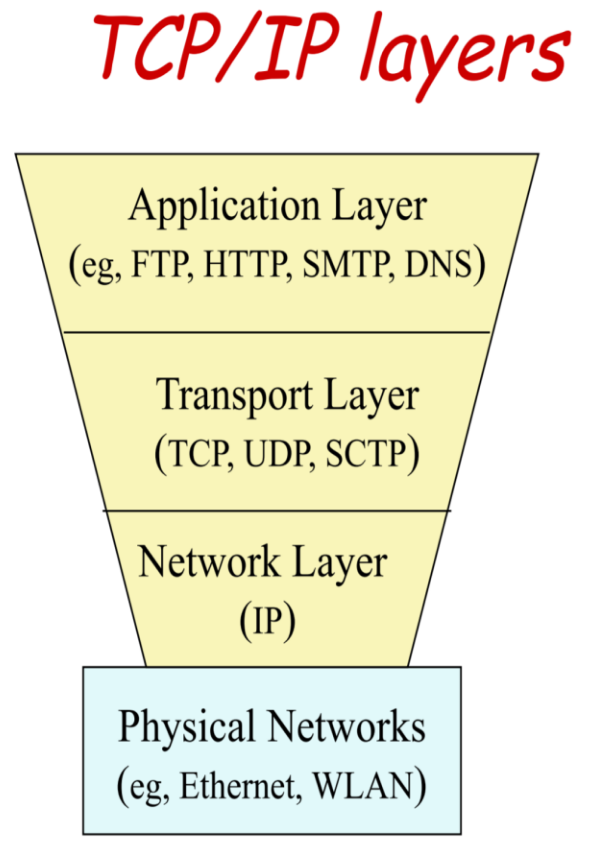
\includegraphics[scale=0.2]{tcp_ip_layers.png}
  \caption{TCP/IP layers}
  \label{fig:tcpiplayers}
\end{figure}

\textbf{Routing in the Internet}

\begin{itemize}
  \item prefix-based routing: IP destination address and network prefix (e.g.
129.13.42) determines physical subnet
  \item change of physical subnet implies change of IP address in order to
have a topological correct address
  \item IP address is bound to a location (\textbf{point of attachment})
\end{itemize}

\textbf{Key Requirements of IP Mobility}

\begin{itemize}
  \item \textbf{Reachability} - A mobile user must remain reachable at all
times via some permanent identifier regardless of its current location
(\textbf{subnet of attachment)}
  \item \textbf{Continuity} - An ongoing communication should not break when
the mobile user moves (across subnet boundaries)
\end{itemize}

\textbf{Desirables requirements}

\begin{itemize}
  \item \textbf{Compatibility} - No changes to current endsystems and routers
required
  \item \textbf{Transparency} - Continuation of communication after
interruption of link possible
  \item \textbf{Efficiency and scalability} - Little or no overhead (typical
connection via low bandwidth radio link)
  \item \textbf{Security} - Authentication of all registration messages
\end{itemize}

\subsection{Problem and possible solution}

None of the layers was designed for mobility.
Mobile devices change IP address while crossing subnets and doesn't remain
reachable anymore.

IP address change breaks transport layer connections, so continuity is
weakened.\\

\textbf{Taxonomy}

\begin{itemize}
  \item Scale: macro, micro
  \item Entities involved in mobility management: mobile-assisted, network-only
  \item Node or group mobility
\end{itemize}

How to handle mobility?\\

\textbf{Change the IP layer} so that the higher layers can still operate
without knowing you have moved (network layer solutions to mobility - e.g.,
MobileIP (v4, v6), GTP) or...

\textbf{Change TCP} so that it can cope (far fronte a) with changing end-point
identifiers (transport layer solutions to mobility - e.g., Mobile TCP, SCTP).

\textbf{Root of the problem and an idea}: the IP address serves as both your
address that is used to locate you, and as your identity that is used to
identify you in TCP connections.

\subsection{Mobile IP}

\begin{figure}[H]
  \centering
  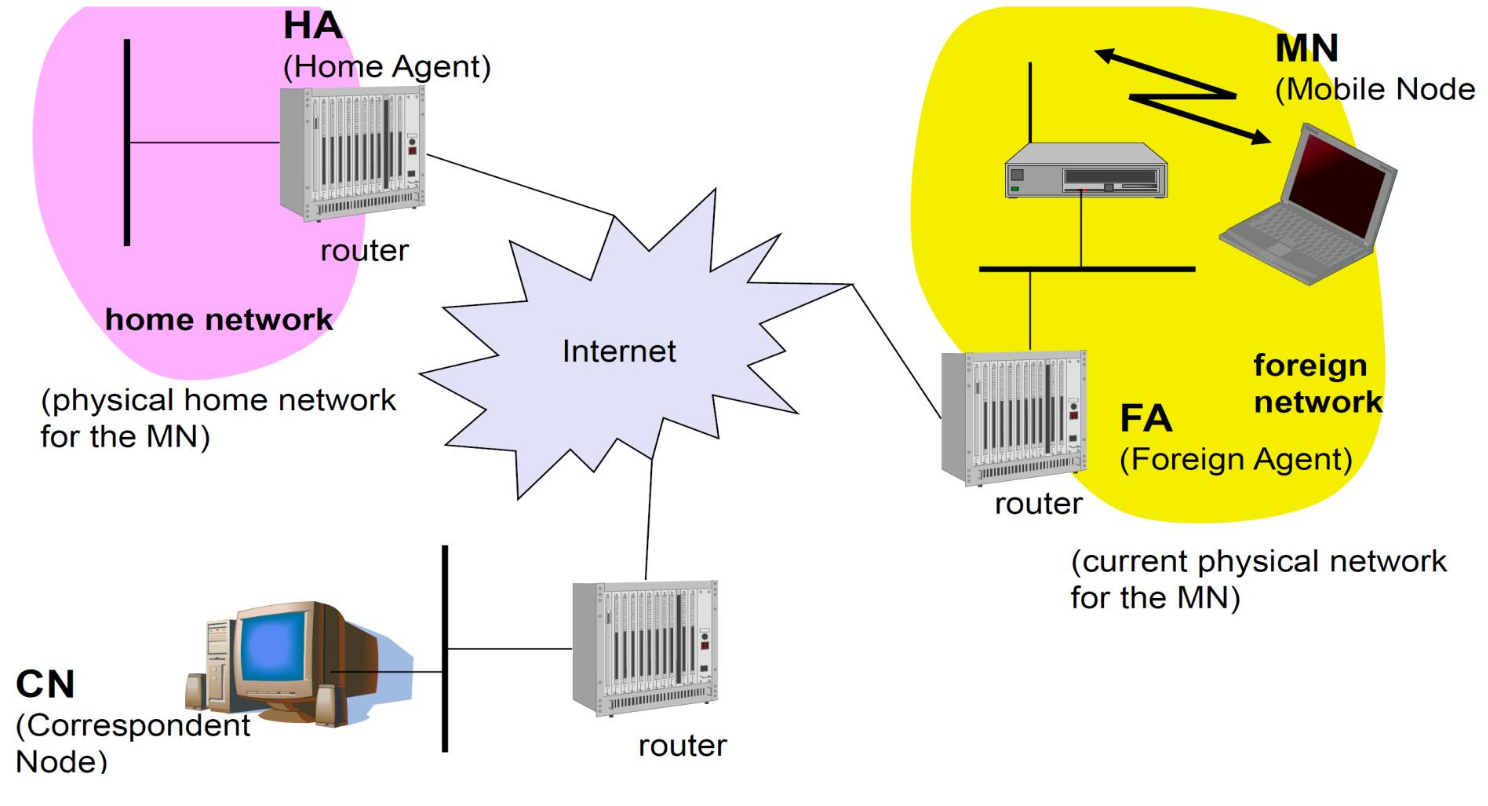
\includegraphics[scale=0.2]{mobileip1.png}
  \caption{Mobile IP example, entities involved}
  \label{fig:mobileip1}
\end{figure}

MN (Mobile Node) moves and senses a network change by listening to periodic
beacons transmitted by the FA (Foreign Agent).

The HA (Home Agent) maintains the binding (home address, care of address,
duration of validity).

Care of address: temporary IP for a mobile device.

\begin{figure}[H]
  \centering
  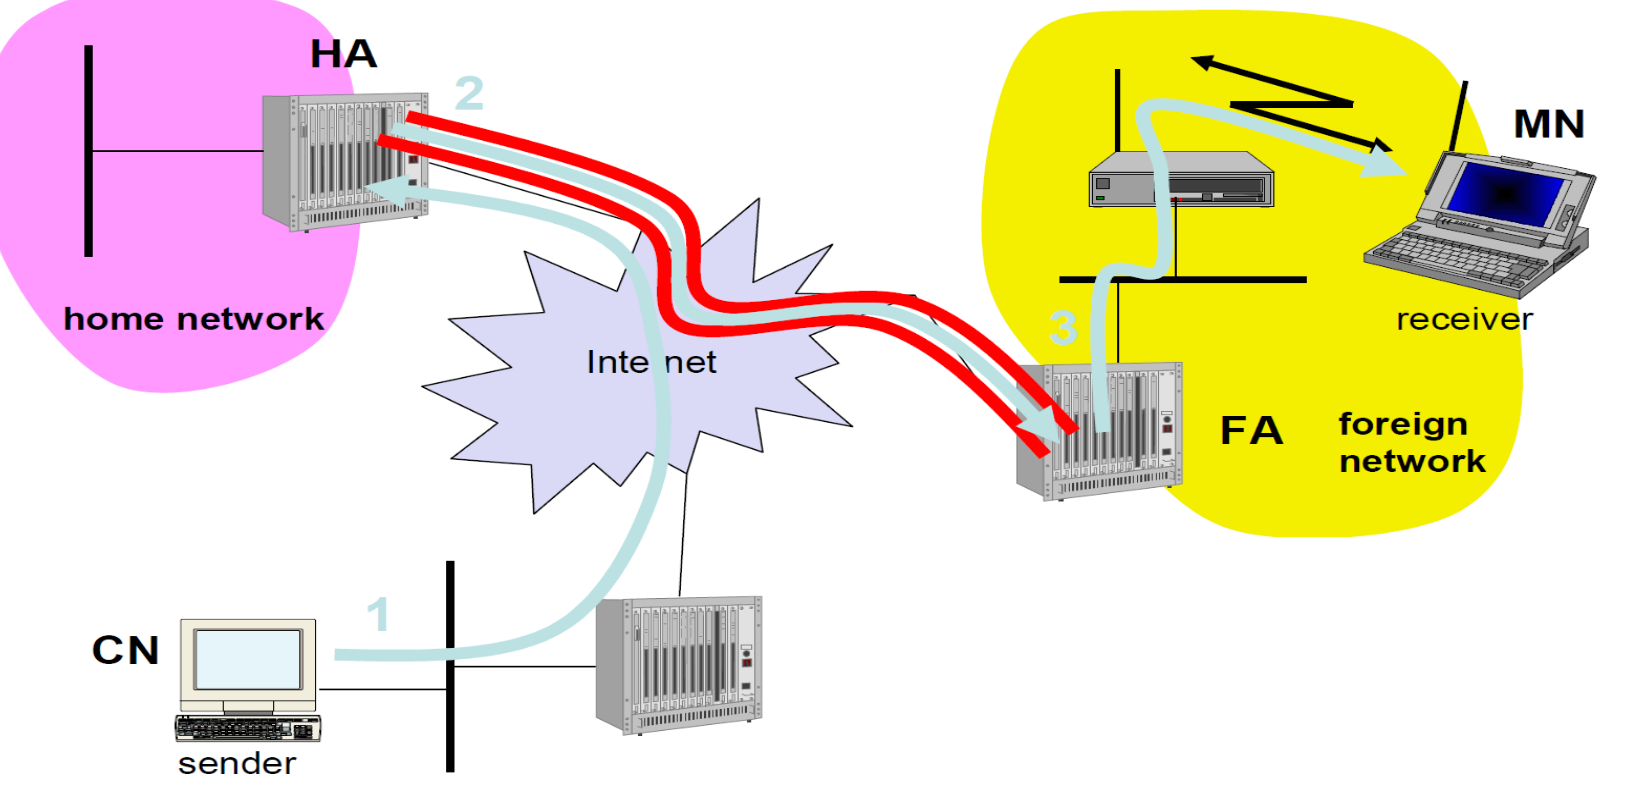
\includegraphics[scale=0.2]{mobileip2.png}
  \caption{Mobile IP example, CN -> MN}
  \label{fig:mobileip2}
\end{figure}

When any packets arrive at the home address, the Home Agent tunnels those
packets to the foreign agent / mobile node at its new address.

IP-in-IP tunneling means that the original IP packet is encapsulated in another
IP packet with the new destination address being the care of address.

\begin{figure}[H]
  \centering
  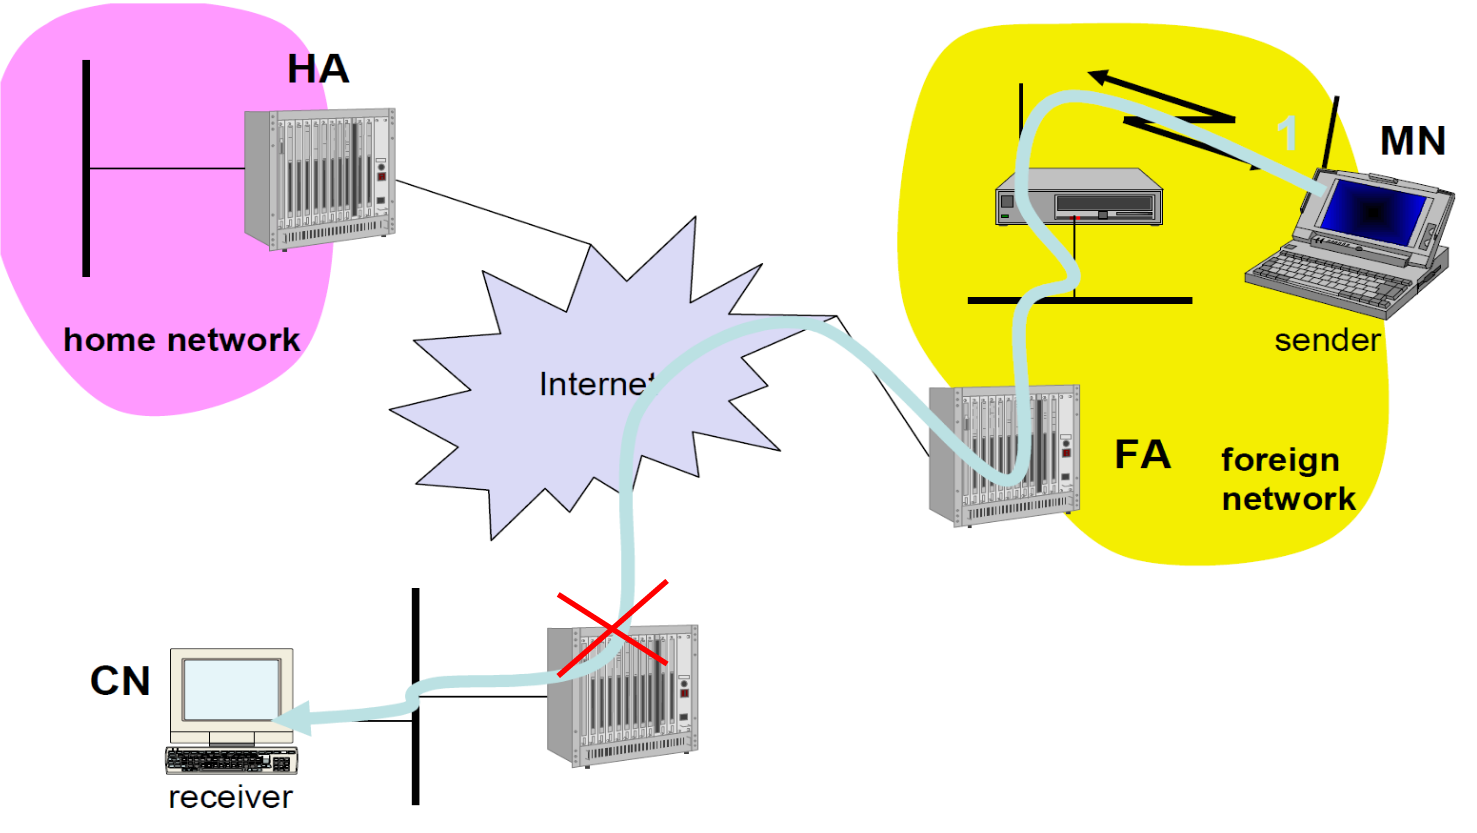
\includegraphics[scale=0.2]{mobileip3.png}
  \caption{Mobile IP example, MN -> CN}
  \label{fig:mobileip3}
\end{figure}

The mobile node can send replies directly, or reverse tunnel (i.e. firewall
scenario) them via home agent.\\

\textbf{Mobile IP - Cons}

\begin{itemize}
  \item \textbf{Security} - Any malicious node can announce a new care of
address and steal packets.
To prevent this, home agent and mobile node must share a secret key and
authenticate their communications
  \item \textbf{Longer routes} - Packets have to travel extra distance
to the home agent and back (triangle routing).
MN could send the care of address (binding) to the CN (Correspondent Node)
which uses it subsequently -> security/privacy issues!
There is also a higher burden on the CN side
  \item \textbf{Ingress filtering at routers}
ISPs can block packets coming from mobile nodes if the source address is their
old home address and does not belong to the IP block of its current network
\end{itemize}

\textbf{Mobile IP - Pros}

\begin{itemize}
  \item Solves mobility at the root (IP is the lowest layer in TCP/IP)
  \item In-built (integrato) tracking support (via permanent IP address and HA)
  \item No change to network core (only edge routers - e.g., HA are affected)
  \item Location privacy (no route optimization)
\end{itemize}

\textbf{Mobile IPv6}

\begin{itemize}
  \item In IPv6, the foreign agent functionality is integrated into the IP
stack of the mobile node itself
  \item Route Optimization is an integral part of the protocol
  \item Built-in security
\end{itemize}

\section{Mobile Cellular Systems}

\subsection{Disambiguation}

\begin{enumerate}
  \item E-UTRA(N) - Evolved UMTS Terrestrial Radio Access (Network)
  \item Super 3G - Is referring to LTE, like WCDMA is referring to UTRA FDD and
TDD
  \item 3.9G - Used to indicate that LTE is not 4G
\end{enumerate}

\textbf{Set of requirements issued by the ITU-R of the ITU in 2008 for what is
marketed as 4G}

\begin{itemize}
  \item Based on an all-Internet Protocol (IP) packet switched network
  \item Interoperability with existing wireless standards
  \item A nominal data rate of 100 Mbit/s (while mobile) and 1 Gbit/s (while
client and station are in relatively fixed positions)
  \item Dynamically share and use the network resources to support more
simultaneous users per cell
  \item Scalable channel bandwidth 5–20 MHz, optionally up to 40 MHz
  \item Peak link spectral efficiency of 15 bit/s/Hz in the downlink, and 6.75
bit/s/Hz in the uplink
  \item Seamless (senza interruzioni) connectivity and global roaming across
multiple networks with smooth handovers (handoff)
  \item System spectral efficiency of up to 3 bit/s/Hz/cell in the downlink and
2.25 bit/s/Hz/cell for indoor usage
  \item Ability to offer high quality of service for multimedia support
\end{itemize}

\begin{figure}[H]
  \centering
  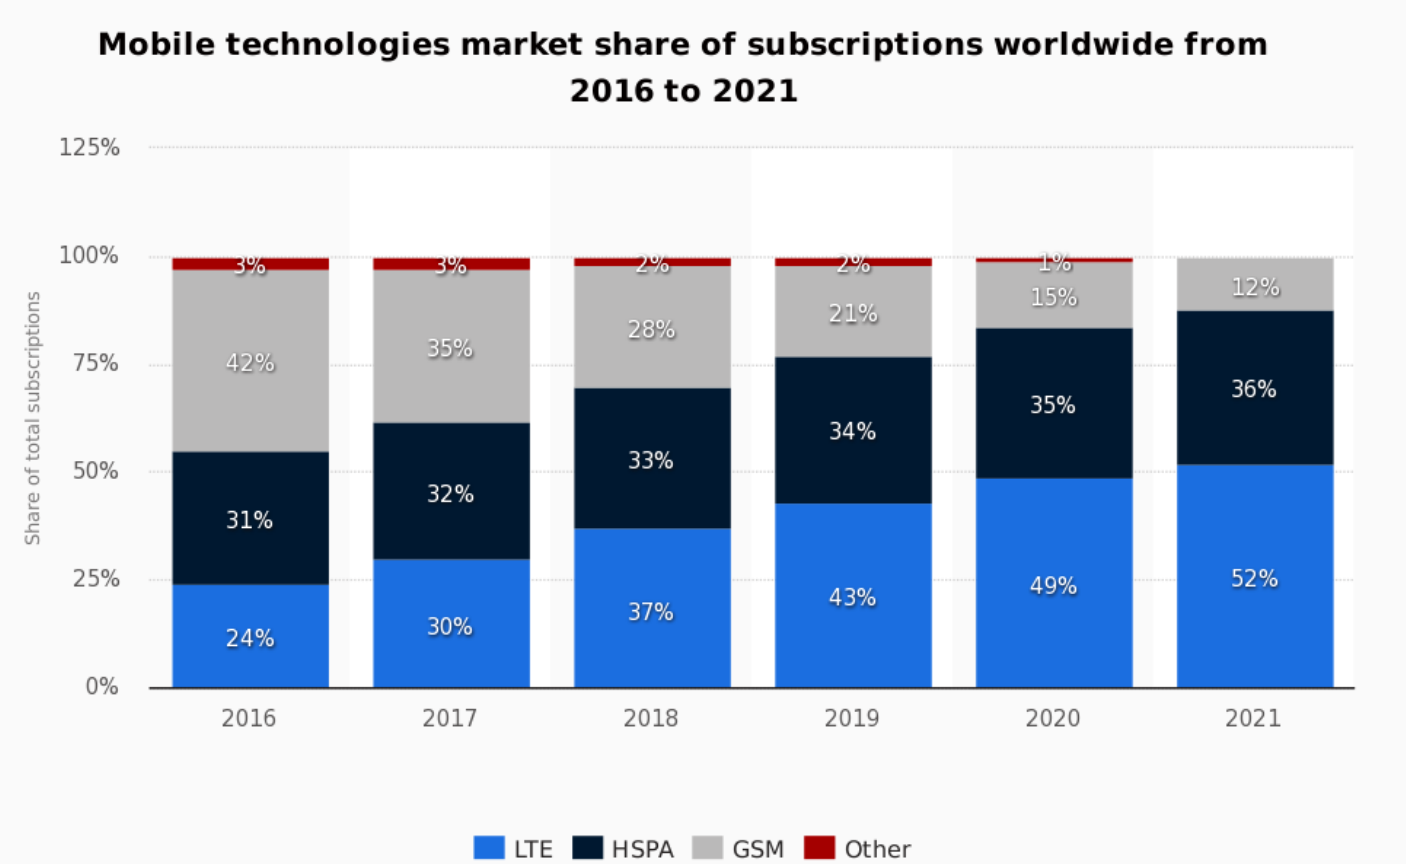
\includegraphics[scale=0.3]{mobtech.png}
  \caption{Mobile technologies market share of subscriptions worldwide from
  2016 to 2011}
  \label{fig:mobtech}
\end{figure}

\subsection{GSM}

\textbf{GSM (Global System for Mobile Communications)} is a standard
developed by the European Telecommunications Standards Institute (ETSI) to
describe the \textbf{protocols for second-generation (2G)} digital cellular
networks used by mobile phones. \\

As of 2014, it has become the de-facto global standard for mobile
communications with over 90\% market share, operating in over 219 countries
and territories.

2G networks developed as a replacement for first generation (1G) analog
cellular networks, and the GSM standard originally described as a digital,
circuit-switched network optimized for full duplex voice telephony. \\

This expanded over time to include data communications, first by
circuit-switched transport, then by packet data transport via GPRS
(General Packet Radio Services) and EDGE (Enhanced Data rates for GSM
Evolution, or EGPRS).

Subsequently, the 3GPP developed third-generation (3G) UMTS standards, followed
by fourth-generation (4G) LTE Advanced standards, which do not form part of the
ETSI GSM standard.

\subsubsection{History...}

\textbf{1982 - Groupe Speciale Mobile is established}

\textbf{1989} - European Telecommunications Standardization Institute
(ETSI) takes over standardization and changes name: Global System for Mobile
(GSM) communication

\textbf{1990} - First Official Commercial launch in Europe

\textbf{1995} - GSM Specifications ported to 1900 MHz band \\

GSM is the most popular 2G technology. Figure \ref{fig:gsm_table} shows its
main characteristics:

\begin{figure}[H]
  \centering
  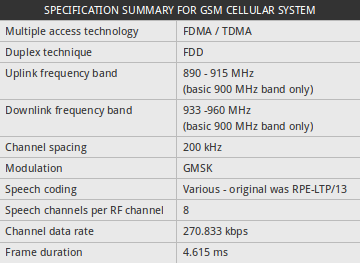
\includegraphics[scale=0.7]{gsm_table.png}
  \caption{Specification Summary for GSM Cellular System }
  \label{fig:gsm_table}
\end{figure}

One of the key features of GSM is the \textbf{Subscriber Identity Module},
commonly known as a SIM card.

The SIM is a detachable smart card containing the user's subscription
information and phone book. This allows the user to retain his or her
information after switching handsets.

Alternatively, the user can also change operators while retaining the handset
simply by changing the SIM. Some operators will block this by allowing the
phone to use only a single SIM, or only a SIM issued by them; this practice
is known as SIM locking.

\subsubsection{GSM – Functional Architecture}

A \textbf{GSM network} comprises of many functional units.
It can be broadly divided into:

\begin{itemize}
  \item \textbf{Base station subsystem} (BSS) - the base stations and their
controllers
  \item \textbf{Network and Switching Subsystem} (NSS) - the part of the
network most similar to a fixed network, sometimes just called the core network
  \item \textbf{GPRS Core Network} (GPRS) - the \textbf{optional} part which
allows packet-based Internet connections (see section \ref{sec:gprs})
  \item \textbf{Operations support system} (OSS) - network maintenance
\end{itemize}

The additional components of the GSM architecture comprise of databases and
\textbf{messaging systems functions}:

\begin{itemize}
  \item VLR : Visitor Location Register
  \item HLR : Home Location Register
  \item AUC : Authentication Center
  \item BTS : Base Transceiver Station
  \item OMC : Operation Maintenance Center
  \item EIR : Equipment Identity Register
\end{itemize}

\begin{figure}[H]
  \centering
  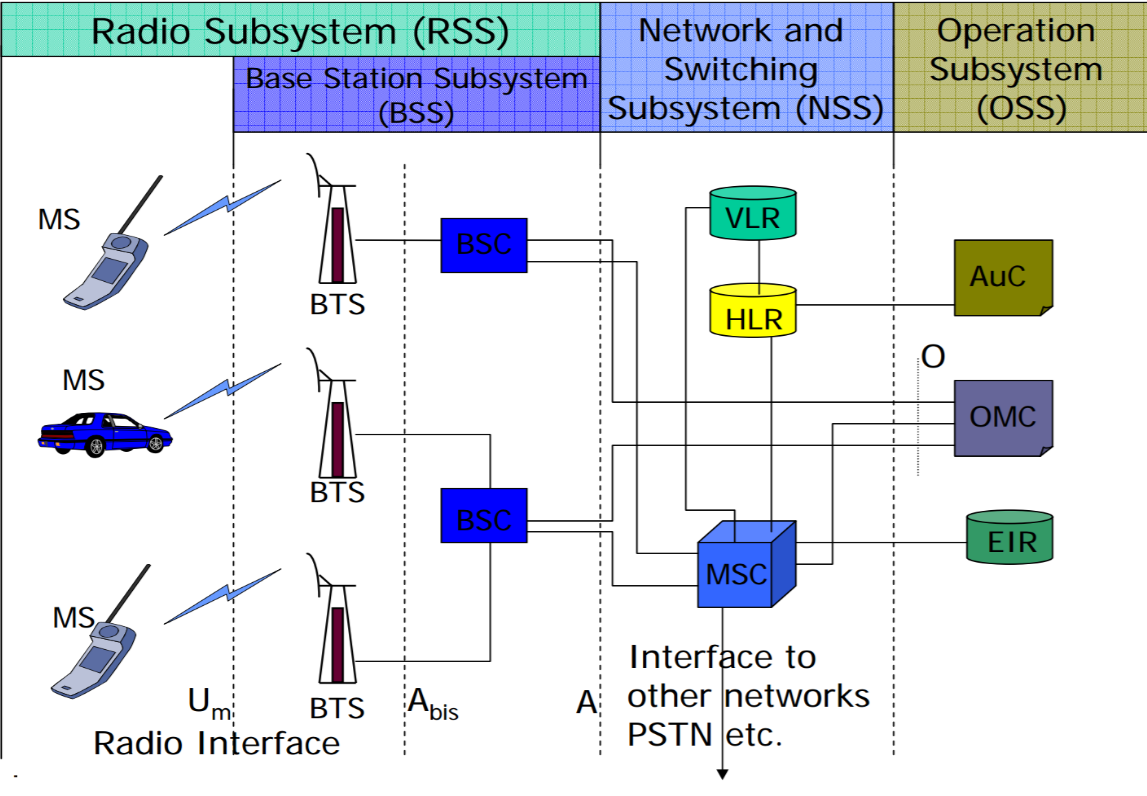
\includegraphics[scale=0.3]{archGSM.png}
  \caption{The structure of a GSM network}
  \label{fig:archGSM}
\end{figure}

The base transceiver stations (BTS) are organised into small groups,
controlled by a base station controller (BSC) which is typically co-located
with one of the BTSs.

The BSC with its associated BTSs is called \textbf{base station subsystem}
(BSS). \\

Further into the core network, there is the main switching area.
This is known as the \textbf{mobile switching centre} (MSC).

Associated with it, there are the \textbf{location registers}, namely the home
location register (HLR) and the visitor location register (VLR) which track
the location of mobiles and enable calls to be routed to them. \\

Additionally there is the \textbf{Authentication Centre} (AuC), and the
Equipment Identify Register (EIR) that are used in authenticating the
mobile before it is allowed onto the network and for billing.

The MS and the BSS communicate across the Um interface (it is the air
interface for the GSM mobile telephone standard, between the mobile station
(MS) and the Base transceiver station (BTS)). It is also known as the air
interface or the radio link.

The BSS communicates with the Network Service Switching (NSS) center across
the A interface.

GSM is a cellular network, which means that cell phones connect to it by
searching for cells in the immediate vicinity. There are five different cell
sizes in a GSM network: \textit{macro, micro, pico, femto, and umbrella} cells.

\section{General Packet Radio Service}
\label{sec:gprs}

General Packet Radio Service (\textbf{GPRS}) is a packet oriented mobile data
service on the 2G and 3G cellular communication system's GSM. It is now
maintained by the 3rd Generation Partnership Project (3GPP).

GPRS usage is typically charged (addebitato) based on volume of data
transferred.

GPRS is a best-effort service, implying variable throughput and latency that
depend on the number of other users sharing the service concurrently, as
opposed to circuit switching, where a certain quality of service (QoS) is
guaranteed during the connection.

In 2G systems, GPRS provides data rates of 56-114 kbit/second. \\

2G cellular technology combined with GPRS is sometimes described as 2.5G,
that is, a technology between the second (2G) and third (3G) generations of
mobile telephony. 2.5G is an attempt to improve data services from
2G.

It connects GSM networks to IP networks (it's basically an overlay network of
data service on 2G networks). Max data rate: 57 Kbps-171 kbit/second.

\subsubsection{GPRS - Quality of Service}
\begin{itemize}
  \item Service precedence (high, normal and low priority groups)
  \item Reliability
  \item Delay
  \item Throughput
\end{itemize}

\subsubsection{LTE – Definitions}

\begin{itemize}
  \item EPC (Evolved Packet Core): the new packet core architecture defined in
3GPP Rel-8
  \item SAE (System Architecture Evolution): the work item within 3GPP for
defining the EPC specifications
  \item LTE (Long Term Evolution): 3GPP work item that developed the radio
access technology and E-UTRAN
  \item EPS (Evolved Packet System): 3GPP term referring to a complete
end-to-end system, that is UE, E-UTRAN and Core Network (EPC)
  \item E-UTRAN - the RAN (radio access network) that implements LTE radio
interface technology
\end{itemize}

\subsection{UMTS - Universal Mobile Telecommunications System}

The Universal Mobile Telecommunications System (\textbf{UMTS}) is a third
generation mobile cellular system for networks based on the GSM standard.

Developed and maintained by the 3GPP, UMTS is a component of the International
Telecommunications Union IMT - 2000 standard set.

UMTS uses wideband code division multiple access (W-CDMA) radio access
technology to offer greater spectral efficiency and bandwidth to mobile network
operators.

UMTS specifies a complete network system, which includes the radio access
network (UMTS Terrestrial Radio Access Network, or UTRAN), the core network
(Mobile Application Part, or MAP) and the authentication of users via SIM
(subscriber identity module) cards.

The technology described in UMTS is sometimes also referred to as 3GSM.

\subsection{User equipment}

In the UMTS and 3GPP LTE, user equipment (UE) is any device used directly by an
end-user to communicate.

It can be a hand-held telephone, a laptop computer equipped with a mobile
broadband adapter, or any other device. \\

User Equipment (UE) comprised of:

\begin{itemize}
  \item Mobile Termination (MT) module (handles all the communication
functions)
  \item Terminal Equipment (TE) module (terminates the data streams)
  \item Universal Integrated Circuit Card (UICC) module (known as the SIM card
for LTE equipment's. It runs an application known as the Universal Subscriber
Identity Module (USIM))
\end{itemize}

\subsection{UTRAN - UMTS Terrestrial Radio Access Network}

Primarily a part of the 3G Mobile Communication Technology and defined as a
collective term for the BTS and Radio Network Controllers which make up the
UMTS radio access network.

Can carry many traffic types from real-time Circuit Switched to IP based Packet
Switched.

The UTRAN allows connectivity between the UE (user equipment) and the core
network.

The UTRAN contains the base stations, which are called Node Bs, and Radio
Network Controllers (RNC).
The RNC provides control functionalities for one or more Node Bs.
A Node B and an RNC can be the same device.

\subsection{E-UTRAN - Evolved Terrestrial Radio Access Network}

E-UTRAN is the network architechture defined for the E-UTRA radio interface as
a part of 3GPP LTE physical layer specification.

It handles radio communications between the mobile and the Evolved Packet Core.

Just one component: the evolved base stations, called \textbf{eNodeB} or eNB.

\begin{figure}[H]
  \centering
  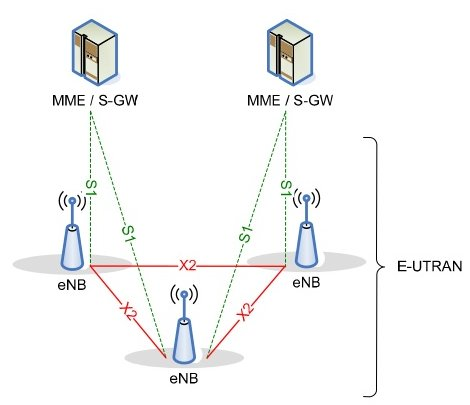
\includegraphics[scale=0.6]{utran_net.jpg}
  \caption{E-UTRAN Architecture}
  \label{fig:utran_net}
\end{figure}

The eBN sends and receives radio transmissions to all the mobiles using the
analogue and digital signal processing functions of the LTE air interface.

The eNB controls the low-level operation of all its mobiles, by sending them
signaling messages such as handover commands.

\subsection{EPC - Evolved Packet Core}

The \textbf{EPC} is the latest evolution of the 3GPP core network architecture.
When designing the evolution of the 3G system, the 3GPP community decided to
use IP (Internet Protocol) as the key protocol to transport all services.
It was therefore agreed that the EPC would not have a circuit-switched domain
anymore and that the EPC should be an evolution of the packet-switched
architecture used in GPRS/UMTS.
This decision had consequences on the architecture itself but also on the way
that the services were provided.
Traditional use of circuits to carry voice and short messages needed to be
replaced by IP-based solutions in the long term.

\begin{figure}[H]
  \centering
  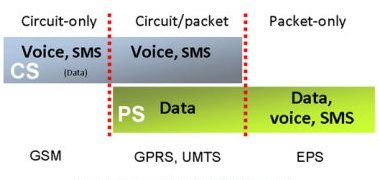
\includegraphics[scale=0.7]{eps.jpg}
  \caption{circuit and packets domains}
  \label{fig:eps}
\end{figure}

\subsubsection{Architecture of the EPC}

The idea of EPC architecture is to handle the payload (the data traffic)
efficiently from performance and costs perspective.

Few network nodes are involved in the handling of the traffic and protocol
conversion is avoided.

It was also decided to separate the user data (also known as the user plane)
and the signalling (also know as the control plane) to make the scaling
independent.
Thanks to this functional split, the operators can dimension and adapt their
network easily.

\begin{figure}[H]
  \centering
  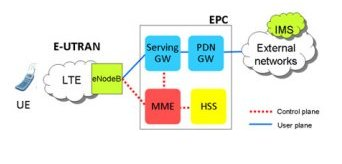
\includegraphics[scale=0.7]{eps_arch.jpg}
  \caption{basic architecture of the EPS when the User Equipment
(UE) is connected to the EPC over E-UTRAN (LTE access network)}
  \label{fig:eps_arch}
\end{figure}

The Evolved NodeB (eNodeB) is the base station for LTE radio.
In figure \ref{fig:eps_arch}, the EPC is composed of four network elements:
the Serving Gateway (Serving GW), the PDN Gateway (PDN GW), the MME and
the HSS.

The EPC is connected to the external networks, which can include the IP
Multimedia Core Network Subsystem (IMS).
